%%%%%%%%%%%%%%%%%%%%%%%%%%%%%%%%%%%%%%%%%%%%%%%%%%%%%%%%%%%%%%%%%
%%%%%%%%%%%%%%%%%%%%%%%%%%%%%%%%%%%%%%%%%%%%%%%%%%%%%%%%%%%%%%%%%
\setcounter{chapter}{4}
\newcommand{\graphicscompanion}{\emph{The \LaTeX{} Graphics Companion}~\cite{graphicscompanion}} 
\newcommand{\hobby}{\emph{A User's Manual for \MP{}}~\cite{metapost}}
\newcommand{\hoenig}{\emph{\TeX{} Unbound}~\cite{unbound}}
\newcommand{\graphicsinlatex}{\emph{Graphics in \LaTeXe{}}~\cite{ursoswald}}

\chapter{Tvorba matematické grafiky}
\label{chap:graphics}

\begin{intro}
Podobně jako zadáváme text, můžeme \LaTeX u zadat pokyny pro vytvoření
grafického výstupu. Možnosti, které při tom
máme, jsou trochu omezené, ale existuje řada \LaTeX ových
rozšíření, které tato omezení překonávají. V~této sekci se o~několika
z~nich dozvíte.
\end{intro}

\section{Úvodní přehled}
Prostředí \ei{picture} umožňuje programování obrázků přímo prostřednictvím
\LaTeX u. Podrobný popis lze nalézt v~\manual. Existují výrazná omezení,
protože sklony úseček stejně jako poloměry kružnic jsou omezené na malou
skupinu hodnot. Na druhou stranu ale \LaTeXe\ prostředí \ei{picture} přináší
příkaz \ci{qbezier} (\uv{\texttt{q}} jako quadratic -- kvadratické).
Kvadratickými Bézierovými
křivkami lze uspokojivě aproximovat mnoho často používaných křivek (např.\
kružnice, elipsy nebo řetězovky), i~když to může vyžadovat trochu
matematické dřiny. Jestliže se navíc pro generování \ci{qbezier} bloků
\LaTeX ových vstupních souborů použije programovací jazyk, např. typu Java, 
prostředí \ei{picture} se stává docela mocným.

Přestože programování obrázků přímo v~\LaTeX u je výrazně omezené
a~často docela únavné, má své výhody. Dokumenty
vytvořené tímto způsobem zabírají méně místa
a~není třeba udržovat žádné grafické soubory.

Balíky, např. \pai{epic} a~\pai{eepic} (popsané např. v~\companion) nebo \pai{pstricks}
pomáhají eliminovat omezení původního prostředí \ei{picture}
a~výrazně posilují grafické schopnosti \LaTeX u.

Zatímco první dva balíky jen obohacují prostředí \ei{picture}, balík \pai{pstricks}
má své vlastní kreslící prostředí, \ei{pspicture}. Síla \pai{pstricks} vychází
z~toho, že tento balík intenzivně využívá možností jazyka \PSi. Mnoho balíků bylo
navíc vytvořeno pro konkrétní použití. Řada z~těchto balíků je detailně popsána
v~\graphicscompanion, neplést si prosím s~\companion.

Asi nejsilnějším grafickým nástrojem spřízněným s~\LaTeX em je \MP, dvojče programu \MF{}
Donalda E. Knutha. \MP\ obsahuje sofistikovaný programovací jazyk \MF u. Na rozdíl
od \MF u~(který generuje bitmapy) generuje \MP\ zapouzdřené \PSi{} soubory,
které mohou být importovány do \LaTeX u. Úvod do programu \MP\ naleznete v~\hobby\ nebo
v~tutoriálu \cite{ursoswald}.

Velmi důkladná diskuze \LaTeX ových a~\TeX ových strategií pro zacházení s~grafikou
(a~fonty) je součástí \hoenig.

\section{Prostředí \texttt{picture}}
\secby{Urs Oswald}{osurs@bluewin.ch}

\subsection{Základní příkazy}

Prostředí \ei{picture}\footnote{Věřte nevěřte, ale prostředí \texttt{picture} je k~dispozici
přímo ve standardním \LaTeXe, není tedy třeba nahrávat žádné speciální balíky.} se vytvoří
jedním z~následujících dvou příkazů
\begin{lscommand}
\ci{begin}\verb|{picture}(|$x,y$\verb|)|\ldots\ci{end}\verb|{picture}|
\end{lscommand}
\noindent nebo
\begin{lscommand}
\ci{begin}\verb|{picture}(|$x,y$\verb|)(|$x_0,y_0$\verb|)|\ldots\ci{end}\verb|{picture}|
\end{lscommand}
Čísla $x,\,y,\,x_0,\,y_0$ jsou odkazy na \ci{unitlength}, které mohou být kdykoliv nastaveny
na původní hodnoty (ale ne uvnitř prostředí \ei{picture}) např. příkazem 
\begin{lscommand}
\ci{setlength}\verb|{|\ci{unitlength}\verb|}{1.2cm}|
\end{lscommand}
Implicitní hodnota \ci{unitlength} je \texttt{1pt}. První pár, $(x,y)$, zajistí v~rámci
dokumentu vynechání obdélníkového místa pro obrázek. Volitelný druhý pár,
$(x_0,y_0)$, přiřadí libovolné souřadnice spodnímu levému rohu vyhrazeného obdélníku.

Většina kreslících příkazů má jednu ze dvou forem
\begin{lscommand}
\ci{put}\verb|(|$x,y$\verb|){|\emph{object}\verb|}|
\end{lscommand}
\noindent nebo
\begin{lscommand}
\ci{multiput}\verb|(|$x,y$\verb|)(|$\Delta x,\Delta y$\verb|){|$n$\verb|}{|\emph{object}\verb|}|\end{lscommand}
Výjimkou jsou Bézierovy křivky, které se kreslí příkazem
\begin{lscommand}
\ci{qbezier}\verb|(|$x_1,y_1$\verb|)(|$x_2,y_2$\verb|)(|$x_3,y_3$\verb|)|
\end{lscommand}
%\newpage



\subsection{Řádkové segmenty}
\begin{example}
\setlength{\unitlength}{5cm}
\begin{picture}(1,1)
  \put(0,0){\line(0,1){1}}
  \put(0,0){\line(1,0){1}}  
  \put(0,0){\line(1,1){1}}  
  \put(0,0){\line(1,2){.5}}
  \put(0,0){\line(1,3){.3333}}
  \put(0,0){\line(1,4){.25}}  
  \put(0,0){\line(1,5){.2}}
  \put(0,0){\line(1,6){.1667}}
  \put(0,0){\line(2,1){1}}
  \put(0,0){\line(2,3){.6667}}
  \put(0,0){\line(2,5){.4}}
  \put(0,0){\line(3,1){1}}  
  \put(0,0){\line(3,2){1}}
  \put(0,0){\line(3,4){.75}}
  \put(0,0){\line(3,5){.6}}
  \put(0,0){\line(4,1){1}}
  \put(0,0){\line(4,3){1}}  
  \put(0,0){\line(4,5){.8}}
  \put(0,0){\line(5,1){1}}
  \put(0,0){\line(5,2){1}}
  \put(0,0){\line(5,3){1}}
  \put(0,0){\line(5,4){1}}
  \put(0,0){\line(5,6){.8333}}
  \put(0,0){\line(6,1){1}}
  \put(0,0){\line(6,5){1}}
\end{picture}
\end{example}
Řádkové segmenty se kreslí příkazem
\begin{lscommand}
\ci{put}\verb|(|$x,y$\verb|){|\ci{line}\verb|(|$x_1,y_1$\verb|){|$length$\verb|}}|
\end{lscommand}
Příkaz \ci{line} má dva argumenty:
\begin{enumerate}
  \item směrový vektor,
  \item délka (\emph{length}).
\end{enumerate}
Komponenty směrového vektoru jsou omezeny na celá čísla
\[
  -6,\,-5,\,\ldots,\,5,\,6,
\]
a~musejí být nesoudělné (nemající kromě jedničky žádného společného dělitele). Obrázek
ukazuje všech dvacet pět možných směrových hodnot v~prvním kvadrantu. Argument délka je
relativní vzhledem k~\ci{unitlength}. Délka je vertikální souřadnice
v~případě vertikálního řádkového segmentu a~horizontální souřadnice ve všech ostatních
případech.

\subsection{Šipky}

\begin{example}
\setlength{\unitlength}{0.75mm}
\begin{picture}(60,40)
  \put(30,20){\vector(1,0){30}}
  \put(30,20){\vector(4,1){20}}
  \put(30,20){\vector(3,1){25}}
  \put(30,20){\vector(2,1){30}}
  \put(30,20){\vector(1,2){10}}
  \thicklines
  \put(30,20){\vector(-4,1){30}}
  \put(30,20){\vector(-1,4){5}}
  \thinlines
  \put(30,20){\vector(-1,-1){5}}
  \put(30,20){\vector(-1,-4){5}}
\end{picture}
\end{example}
Šipky se kreslí příkazem
\begin{lscommand}
\ci{put}\verb|(|$x,y$\verb|){|\ci{vector}\verb|(|$x_1,y_1$\verb|){|$length$\verb|}}|
\end{lscommand}
Hodnoty směrových vektorů šipek jsou omezeny ještě více než u~řádkových segmentů,
konkrétně se jedná o~celá čísla
\[
  -4,\,-3,\,\ldots,\,3,\,4.
\]
Opět platí, že komponenty musí být nesoudělné. Všimněte si efektu příkazu \ci{thicklines}
na šipky ukazující nahoru doleva.

\subsection{Kružnice}

\begin{example}
\setlength{\unitlength}{1mm}
\begin{picture}(60, 40)
  \put(20,30){\circle{1}}
  \put(20,30){\circle{2}}
  \put(20,30){\circle{4}}
  \put(20,30){\circle{8}}
  \put(20,30){\circle{16}}
  \put(20,30){\circle{32}}
  
  \put(40,30){\circle{1}}
  \put(40,30){\circle{2}}
  \put(40,30){\circle{3}}
  \put(40,30){\circle{4}}
  \put(40,30){\circle{5}}
  \put(40,30){\circle{6}}
  \put(40,30){\circle{7}}
  \put(40,30){\circle{8}}
  \put(40,30){\circle{9}}
  \put(40,30){\circle{10}}
  \put(40,30){\circle{11}}
  \put(40,30){\circle{12}}
  \put(40,30){\circle{13}}
  \put(40,30){\circle{14}}
  
  \put(15,10){\circle*{1}}
  \put(20,10){\circle*{2}}
  \put(25,10){\circle*{3}}
  \put(30,10){\circle*{4}}
  \put(35,10){\circle*{5}}
\end{picture}
\end{example}
Příkaz
\begin{lscommand}
  \ci{put}\verb|(|$x,y$\verb|){|\ci{circle}\verb|{|\emph{diameter}\verb|}}|
\end{lscommand}
\noindent nakreslí kružnici se středem $(x,y)$ a~průměrem (ano, nikoliv poloměrem) \emph{diameter}.
Maximální průměr, který prostředí \ei{picture} akceptuje, je zhruba 14\,mm,
ale použít nelze ani některé menší průměry. Příkaz \ci{circle*} nakreslí disky
(vyplněné kružnice).

Podobně jako u~řádkových segmentů je možno použít přídavné balíky, např.
\pai{eepic} nebo \pai{pstricks}. Tyto balíky jsou důkladně popsány
v~\graphicscompanion.

Kdo se nebojí provádět (sám nebo pomocí programu) nezbytné výpočty, může
v~prostředí \ei{picture} z~kvadratických B\'ezierových křivek složit dohromady
libovolné kružnice a~elipsy. Příklady a~zdrojové soubory v~Javě jsou
uvedeny v~\graphicsinlatex.


\subsection{Text a~vzorce}

\begin{example}
\setlength{\unitlength}{0.8cm}
\begin{picture}(6,5)
  \thicklines
  \put(1,0.5){\line(2,1){3}}
  \put(4,2){\line(-2,1){2}}
  \put(2,3){\line(-2,-5){1}}
  \put(0.7,0.3){$A$}
  \put(4.05,1.9){$B$}
  \put(1.7,2.95){$C$}
  \put(3.1,2.5){$a$}
  \put(1.3,1.7){$b$}
  \put(2.5,1.05){$c$}
  \put(0.3,4){$F=
    \sqrt{s(s-a)(s-b)(s-c)}$}  
  \put(3.5,0.4){$\displaystyle
    s:=\frac{a+b+c}{2}$}
\end{picture}
\end{example}
Jak ukazuje tento příklad, text a~vzorce mohou být obvyklým způsobem vepsány do prostředí
\ei{picture} pomocí příkazu \ci{put}.

\subsection{\ci{multiput} a~\ci{linethickness}}

\begin{example}
\setlength{\unitlength}{2mm}
\begin{picture}(30,20)
  \linethickness{0.075mm}
  \multiput(0,0)(1,0){26}%
    {\line(0,1){20}}
  \multiput(0,0)(0,1){21}%
    {\line(1,0){25}}
  \linethickness{0.15mm}    
  \multiput(0,0)(5,0){6}%
    {\line(0,1){20}}
  \multiput(0,0)(0,5){5}%
    {\line(1,0){25}}
  \linethickness{0.3mm}    
  \multiput(5,0)(10,0){2}%
    {\line(0,1){20}}
  \multiput(0,5)(0,10){2}%
    {\line(1,0){25}}
\end{picture}
\end{example}
Příkaz
\begin{lscommand}
  \ci{multiput}\verb|(|$x,y$\verb|)(|$\Delta x,\Delta y$\verb|){|$n$\verb|}{|\emph{object}\verb|}|
\end{lscommand}
\noindent má 4 argumenty: počáteční bod, vektor pro překlad z~jednoho objektu
do jiného, počet objektů a~objekt, který se má nakreslit. 

Příkaz \ci{linethickness}
se vztahuje na horizontální a~vertikální linkové segmenty, ale ne na šikmé linkové segmenty
ani kružnice. \ci{linethickness} se také vztahuje na kvadratické B\'ezierovy křivky!

\subsection{Ovály}

\begin{example}
\setlength{\unitlength}{0.75cm}
\begin{picture}(6,4)
  \linethickness{0.075mm}
  \multiput(0,0)(1,0){7}%
    {\line(0,1){4}}
  \multiput(0,0)(0,1){5}%
    {\line(1,0){6}}
  \thicklines
  \put(2,3){\oval(3,1.8)} 
  \thinlines
  \put(3,2){\oval(3,1.8)} 
  \thicklines
  \put(2,1){\oval(3,1.8)[tl]} 
  \put(4,1){\oval(3,1.8)[b]} 
  \put(4,3){\oval(3,1.8)[r]} 
  \put(3,1.5){\oval(1.8,0.4)}     
\end{picture}
\end{example}
Příkaz
\begin{lscommand}
  \ci{put}\verb|(|$x,y$\verb|){|\ci{oval}\verb|(|$w,h$\verb|)}|
\end{lscommand}
\noindent nebo
\begin{lscommand}
  \ci{put}\verb|(|$x,y$\verb|){|\ci{oval}\verb|(|$w,h$\verb|)[|\emph{position}\verb|]}|
\end{lscommand}
\noindent nakreslí ovál se středem $(x,y)$, šířkou $w$ a~výškou $h$. Volitelné \emph{poziční}
argumenty \texttt{b}, \texttt{t}, \texttt{l}, \texttt{r} se vztahují
k~\uv{horní}, \uv{spodní}, \uv{levé} a~\uv{pravé} straně a~mohou být kombinovány,
jak je ukázáno na obrázku. 

Šířku čar je možno upravovat buď příkazem \ci{linethickness}\verb|{|\emph{length}\verb|}| nebo příkazy
\ci{thinlines} a~\ci{thicklines}. \ci{linethickness}\verb|{|\emph{length}\verb|}|
se vztahuje jen na horizontální a~vertikální čáry (a~kvadratické B\'ezierovy křivky),
zatímco \ci{thinlines} a~\ci{thicklines} lze navíc použít na šikmé čárové segmenty, kružnice a~ovály.

\subsection{Vícenásobné použití předdefinovaných boxů s~obrázky}

\begin{example}
\setlength{\unitlength}{0.5mm}
\begin{picture}(120,168)
\newsavebox{\foldera}
\savebox{\foldera}
  (40,32)[bl]{% definition 
  \multiput(0,0)(0,28){2}
    {\line(1,0){40}}
  \multiput(0,0)(40,0){2}
    {\line(0,1){28}}
  \put(1,28){\oval(2,2)[tl]}
  \put(1,29){\line(1,0){5}}
  \put(9,29){\oval(6,6)[tl]}
  \put(9,32){\line(1,0){8}}
  \put(17,29){\oval(6,6)[tr]}
  \put(20,29){\line(1,0){19}}
  \put(39,28){\oval(2,2)[tr]}  
}
\newsavebox{\folderb}
\savebox{\folderb}
  (40,32)[l]{% definition 
  \put(0,14){\line(1,0){8}}
  \put(8,0){\usebox{\foldera}}
}
\put(34,26){\line(0,1){102}} 
\put(14,128){\usebox{\foldera}}
\multiput(34,86)(0,-37){3}
  {\usebox{\folderb}} 
\end{picture}
\end{example}
Box s~obrázkem je možno \emph{deklarovat} příkazem
\begin{lscommand}
  \ci{newsavebox}\verb|{|\emph{name}\verb|}|
\end{lscommand}
\noindent a~následně \emph{definovat} pomocí
\begin{lscommand}
  \ci{savebox}\verb|{|\emph{name}\verb|}(|\emph{width,height}\verb|)[|\emph{position}\verb|]{|\emph{content}\verb|}|
\end{lscommand}
\noindent a~potom \emph{vykreslit} libovolně mnohokrát pomocí
\begin{lscommand}
  \ci{put}\verb|(|$x,y$\verb|){|\ci{usebox}\verb|{|\emph{name}\verb|}}|
\end{lscommand}
Nepovinný parametr \emph{position} specifikuje \emph{referenční bod} saveboxu.
V~našem příkladu je tento parameter specifikován hodnotou \texttt{bl}, což
umístí referenční bod do spodního levého rohu saveboxu (\texttt{b}ottom -- spodní část
a~\texttt{l}eft~\discretionary{--}{--}{--}~vlevo). Zbylé hodnoty,
ze kterých je možno složit specifikaci pozice, jsou \texttt{t} (\texttt{t}op -- horní část)
a~\texttt{r} (\texttt{r}ight -- vpravo).

Argument \emph{name} se odkazuje na \LaTeXe ové \uv{skladiště materiálu}
a~má proto charakter příkazu, proto jsou v~našem příkladu zpětná lomítka. Boxy nesoucí
obrázky mohou být vnořené: v~našem příkladě je použito \ci{foldera} uvnitř definice
\ci{folderb}.

Museli jsme použít příkaz \ci{oval}, protože příkaz \ci{line} nefunguje, pokud je délka
segmentu menší než zhruba 3\,mm.

\subsection{Kvadratické B\'ezierovy křivky}

\begin{example}
\setlength{\unitlength}{0.8cm}
\begin{picture}(6,4)
  \linethickness{0.075mm}
  \multiput(0,0)(1,0){7}
    {\line(0,1){4}}
  \multiput(0,0)(0,1){5}
    {\line(1,0){6}}
  \thicklines
  \put(0.5,0.5){\line(1,5){0.5}}    
  \put(1,3){\line(4,1){2}} 
  \qbezier(0.5,0.5)(1,3)(3,3.5)
  \thinlines   
  \put(2.5,2){\line(2,-1){3}}
  \put(5.5,.5){\line(-1,5){.5}}
  \linethickness{1mm}
  \qbezier(2.5,2)(5.5,0.5)(5,3)
  \thinlines
  \qbezier(4,2)(4,3)(3,3)
  \qbezier(3,3)(2,3)(2,2)
  \qbezier(2,2)(2,1)(3,1)
  \qbezier(3,1)(4,1)(4,2)
\end{picture}
\end{example}
Jak tento příklad ukazuje, rozdělení kružnice na čtyři kvadratické B\'ezierovy křivky
nevede k~uspokojivému výsledku. Křivek je potřeba alespoň osm. Obrázek opět ukazuje
efekt příkazu \ci{linethickness} na horizontální a~vertikální čáry a~příkazů
\ci{thinlines} a~\ci{thicklines} na šikmé čárové segmenty. Ukazuje také, že oba
typy příkazů ovlivňují kvadratické B\'ezierovy křivky, každý z~příkazů \uv{přepisující}
nastavení toho předchozího.

Nechť $P_1=(x_1,\,y_1),\,P_2=(x_2,\,y_2)$ značí koncové body a~$m_1,\,m_2$ 
příslušné sklony kvadratické B\'ezierovy křivky. Střední kontrolní bod
$S=(x,\,y)$ potom splňuje rovnici
\begin{equation} \label{zwischenpunkt}
  \left\{
    \begin{array}{rcl}
      x & = & \displaystyle \frac{m_2 x_2-m_1x_1-(y_2-y_1)}{m_2-m_1}, \\
      y & = & y_i+m_i(x-x_i)\qquad (i=1,\,2).
    \end{array}
  \right.
\end{equation}
\noindent \graphicsinlatex\ obsahuje Javový program, který generuje nezbytnou
příkazovou řádku pro \ci{qbezier}.

\subsection{Řetězovka}

\begin{example}
\setlength{\unitlength}{1cm}
\begin{picture}%
   (4.3,3.6)(-2.5,-0.25)
\put(-2,0){\vector(1,0){4.4}}
\put(2.45,-.05){$x$}
\put(0,0){\vector(0,1){3.2}}
\put(0,3.35){\makebox(0,0){$y$}}
\qbezier(0.0,0.0)(1.2384,0.0)
  (2.0,2.7622) 
\qbezier(0.0,0.0)(-1.2384,0.0)
  (-2.0,2.7622)
\linethickness{.075mm}
\multiput(-2,0)(1,0){5}
  {\line(0,1){3}}
\multiput(-2,0)(0,1){4}
  {\line(1,0){4}}
\linethickness{.2mm}
\put( .3,.12763){\line(1,0){.4}}
\put(.5,-.07237){\line(0,1){.4}}
\put(-.7,.12763){\line(1,0){.4}}
\put(-.5,-.07237){\line(0,1){.4}}
\put(.8,.54308){\line(1,0){.4}}
\put(1,.34308){\line(0,1){.4}}
\put(-1.2,.54308){\line(1,0){.4}}
\put(-1,.34308){\line(0,1){.4}}
\put(1.3,1.35241){\line(1,0){.4}}
\put(1.5,1.15241){\line(0,1){.4}}
\put(-1.7,1.35241){\line(1,0){.4}}
\put(-1.5,1.15241){\line(0,1){.4}}
\put(-2.5,-0.25){\circle*{0.2}}
\end{picture}
\end{example}
Každá ze symetrických polovin paraboly $y=\cosh x-1$ na tomto obrázku lze přibližně získat
pomocí B\'ezierovy křivky. Pravá polovina křivky končí v~bodě \((2,\,2.7622)\), kde má
sklon hodnotu \(m=3.6269\). Pokud opět použijeme rovnici (\ref{zwischenpunkt}), můžeme
vypočítat střední kontrolní body, které v~našem případě jsou $(1.2384,\,0)$ a~$(-1.2384,\,0)$. 
Křížky značí body \emph{skutečné} paraboly. Chyba, menší než jedno procento, je stěží postřehnutelná.

V~následujícím příkladu je u~\verb|\begin{picture}| použit nepovinný parametr.
Obrázek se definuje pomocí vhodných \uv{matematických} souřadnic, zatímco příkazem
\begin{lscommand} 
  \ci{begin}\verb|{picture}(4.3,3.6)(-2.5,-0.25)|
\end{lscommand}
\noindent přiřadíme levému dolnímu rohu (viz černý kotouč) souřadnice $(-2.5,-0.25)$. 

\subsection{Rychlost ve speciální teorii relativity}

\begin{example}
\setlength{\unitlength}{0.8cm}
\begin{picture}(6,4)(-3,-2)
  \put(-2.5,0){\vector(1,0){5}}
  \put(2.7,-0.1){$\chi$}
  \put(0,-1.5){\vector(0,1){3}}
  \multiput(-2.5,1)(0.4,0){13}
    {\line(1,0){0.2}}
  \multiput(-2.5,-1)(0.4,0){13}
    {\line(1,0){0.2}}
  \put(0.2,1.4)
    {$\beta=v/c=\tanh\chi$}
  \qbezier(0,0)(0.8853,0.8853)
    (2,0.9640)
  \qbezier(0,0)(-0.8853,-0.8853)
    (-2,-0.9640)
  \put(-3,-2){\circle*{0.2}}
\end{picture}
\end{example}
Kontrolní body obou B\'ezierových křivek byly získány pomocí vzorců (\ref{zwischenpunkt}).
Kladná část se určí pomocí $P_1=(0,\,0)$, $m_1=1$, $P_2=(2,\,\tanh 2)$ a~$m_2=1/\cosh^2 2$.
Obrázek je opět definován pomocí vhodných souřadnic a~levému dolnímu rohu
jsou přiřazeny matematické souřadnice $(-3,-2)$, to je onen černý kotouč.

\section{Grafický balík Ti\emph{k}Z \& PGF}
V~dnešní době umí každý systém generující \LaTeX ový výstup vytvořit pěknou
vektorovou grafiku, jen rozhraní se poněkud liší. Balík PGF poskytuje abstraktní
vrstvu nad těmito rozhraními a~umožňuje používat jednoduché příkazy
pro vytvoření složité vektorové grafiky přímo \uv{zevnitř} \LaTeX ového dokumentu.
Balík PGF obsahuje více než sedmisetstránkovou dokumentaci~\cite{pgfplot}, 
my si však dovolíme být v~této sekci o~pár set stran stručnější. 
%my proto v~této sekci budeme struční.

Pro přístup k~funkcím \uv{vyšší úrovně} balíku PGF byste si měli nahrát
balík \pai{tikz}, s~kterým můžete používat výkonné příkazy ke kreslení grafiky
přímo ze svého dokumentu. Kreslící instrukce vložte dovnitř prostředí \ei{tikzpicture}.

\begin{example}
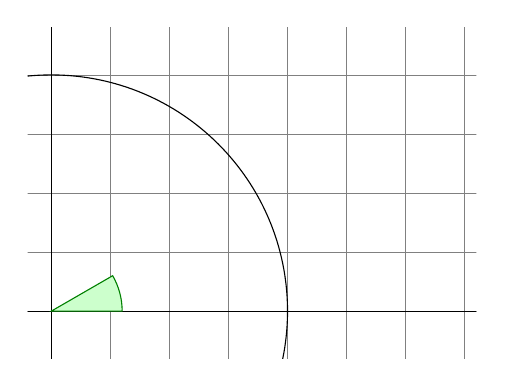
\begin{tikzpicture}[scale=3]
  \clip (-0.1,-0.2)
     rectangle (1.8,1.2);
  \draw
     [step=.25cm,gray,very thin]
     (-1.4,-1.4) grid (3.4,3.4);
  \draw (-1.5,0) -- (2.5,0);
  \draw (0,-1.5) -- (0,1.5);
  \draw (0,0) circle (1cm);
  \filldraw[fill=green!20!white,
            draw=green!50!black]
    (0,0) -- (3mm,0mm) 
        arc (0:30:3mm) -- cycle;
\end{tikzpicture}
\end{example}
Pokud jste obeznámeni s~dalšími programovacími jazyky, možná si všimnete
povědomého středníku (\texttt{;}) použitého k~oddělení příkazů. 

Pomocí
příkazu \ci{usetikzlibrary} v~preambuli můžete aktivovat řadu rozšiřujících
rysů pro kreslení speciálních tvarů, např. tento box, který je trochu prohnutý.
\begin{example}
\usetikzlibrary{%
  decorations.pathmorphing}
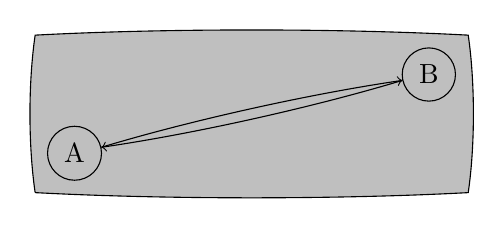
\begin{tikzpicture}[
   decoration={bent,aspect=.3}]
 \draw [decorate,fill=lightgray]
        (0,0) rectangle (5.5,2);
 \node[circle,draw] 
        (A) at (.5,.5) {A};
 \node[circle,draw] 
        (B) at (5,1.5) {B};
 \draw[->,decorate] (A) -- (B);
 \draw[->,decorate] (B) -- (A);
\end{tikzpicture}
\end{example}

Můžete dokonce kreslit diagramy, které jako by vypadly z~knihy o~programování
v~Pascalu. Kód takového diagramu je rozsáhlejší než v~předchozím příkladu,
takže ukážeme jenom výsledek. V~PGF dokumentaci je důkladný popis kresby
tohoto diagramu.

\begin{center}
\begin{tikzpicture}[point/.style={coordinate},thick,draw=black!50,>=stealth',
                    tip/.style={->,shorten >=1pt},every join/.style={rounded corners},
                    skip loop/.style={to path={-- ++(0,#1) -| (\tikztotarget)}},
                    hv path/.style={to path={-| (\tikztotarget)}},
                    vh path/.style={to path={|- (\tikztotarget)}},
                 terminal/.style={
            rounded rectangle,
            minimum size=6mm,
            thick,draw=black!50,
            top color=white,bottom color=black!20,
            font=\ttfamily\tiny},
                nonterminal/.style={
                       rectangle,
                       minimum size=6mm,
                       thick,
                       draw=red!50!black!50,         % 50% red and 50% black,
                       top color=white,              % a shading that is white at the top...
                       bottom color=red!50!black!20, % and something else at the bottom
                       font=\itshape\tiny}]
\matrix[column sep=3mm] {
  % First row:
  & & & & & & & & & & & \node (plus) [terminal] {+};\\
  % Second row:
  \node (p1) [point] {}; &     \node (ui1)    [nonterminal] {unsigned integer}; &
  \node (p2) [point] {}; &     \node (dot)    [terminal]    {.};                &
  \node (p3) [point] {}; &     \node (digit) [terminal]     {digit};            &
  \node (p4) [point] {}; &     \node (p5)     [point] {};                       &
  \node (p6) [point] {}; &     \node (e)      [terminal]    {E};                &
  \node (p7) [point] {}; &                                                      &
  \node (p8) [point] {}; &     \node (ui2)    [nonterminal] {unsigned integer}; &
  \node (p9) [point] {}; &     \node (p10)    [point]       {};\\
  % Third row:
  & & & & & & & & & & & \node (minus)[terminal] {-};\\
};
{ [start chain]
  \chainin (p1);
  \chainin (ui1)   [join=by tip];
  \chainin (p2)    [join];
  \chainin (dot)   [join=by tip];
  \chainin (p3)    [join];
  \chainin (digit) [join=by tip];
  \chainin (p4)    [join];
  { [start branch=digit loop]
    \chainin (p3) [join=by {skip loop=-6mm,tip}];
  }
  \chainin (p5)    [join,join=with p2 by {skip loop=6mm,tip}];
  \chainin (p6)    [join];
  \chainin (e)     [join=by tip];
  \chainin (p7)    [join];
  { [start branch=plus]
    \chainin (plus) [join=by {vh path,tip}];
    \chainin (p8)    [join=by {hv path,tip}];
  }
  { [start branch=minus]
    \chainin (minus) [join=by {vh path,tip}];
    \chainin (p8)    [join=by {hv path,tip}];
  }
  \chainin (p8)    [join];
  \chainin (ui2)   [join=by tip];
  \chainin (p9)    [join,join=with p6 by {skip loop=-11mm,tip}];
  \chainin (p10)   [join=by tip];
}
\end{tikzpicture}
\end{center}

\pagebreak
Potřebujete-li kreslit grafy číselných hodnot nebo funkcí, měli
byste se důkladněji seznámit s~balíky \pai{pgfplots} a~\pai{pgfplotstable}, které poskytují
všechno potřebné. Vyhodnocení funkcí, které chcete zobrazit, umí
dokonce udělat vyvoláním externího programu \texttt{gnuplot}, \url{http://www.gnuplot.info/}.

Pro ještě náročnější čtenáře zmiňujeme existenci jazyka~R -- výpočetní prostředí zaměřené na statistiku, \url{http://www.r-project.org/}, a~pomocného balíku \textsf{Sweave}. 

Nelze opominout též systém Sage -- prostředí zaměřené na matematiku, \url{http://www.sagemath.org/}, a~pomocný balík Sage\TeX, kde má našinec na vývoji a~testování nemalé zásluhy (Robert Mařík, Brno).

%%% Local Variables:
%%% TeX-master: "lshort.tex"
%%% mode: flyspell
%%% TeX-PDF-mode: t
%%% End:
